\section{Team Maintenance}

Managing Teams
\newline\newline
In murcs teams are groups of people who will work together on certain projects. The team will include information such as the short and long name of the team, a list of all the members in the team and the ability to add and remove members and a method of setting the product owner and scrum master of the project and the ability to view peer programming hours within the team.
\newline
Firstly in order to create a team there are two methods, very similar to people, you either use the toolbar creation button or select File->New->Team. Both of these methods will open up a create team dialog as displayed below.

\begin{figure}[H]
\centering
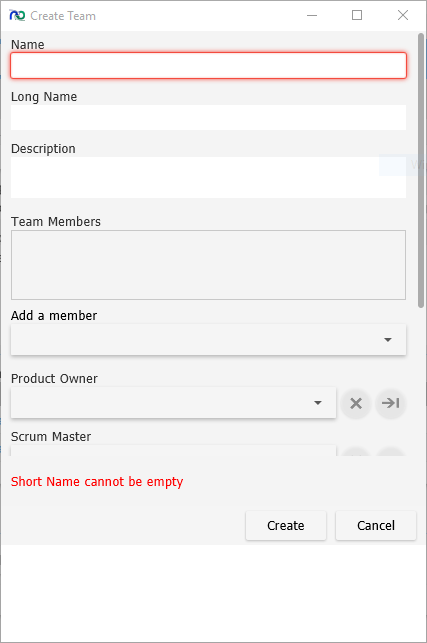
\includegraphics[width=\textwidth]{images/screenshots/teams1.PNG}
\caption{Creating a Team}
\label{fig:new_project}
\end{figure}

Once this has appeared you need to enter a name for the team, this is the only compulsory field. The other fields can be filled in and to add team members simply select from the drop down box of members in the add team member drop down box, as shown below. After selecting someone they will appear in the Team Members area and to then remove them simply click the X box next to the person.

\begin{figure}[H]
\centering
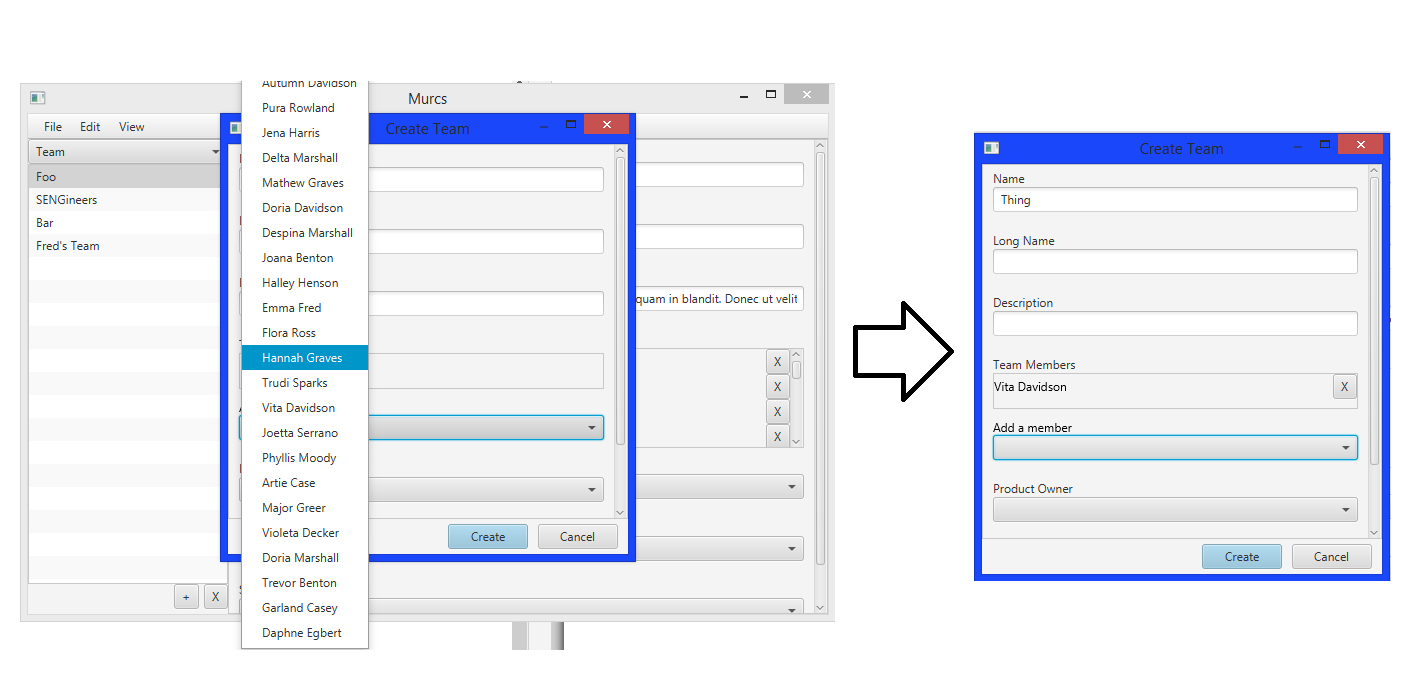
\includegraphics[width=\textwidth]{images/screenshots/teams2.PNG}
\caption{Adding People to a Team}
\label{fig:new_project}
\end{figure}

Once you finished editing the values you want simply press the create button. If there are any problems creating the team (usually if you haven't filled in a necessary field) then the team will not be created and you will get an error message at the bottom of the creation window as shown below.

\begin{figure}[H]
\centering
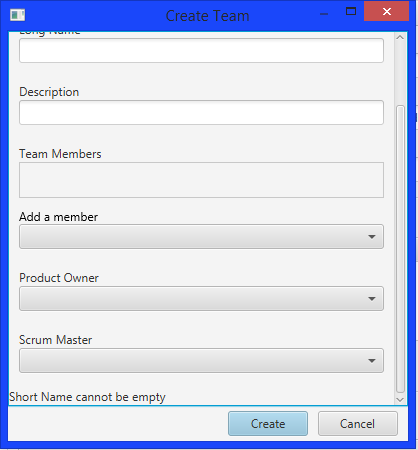
\includegraphics[width=\textwidth]{images/screenshots/teams3.PNG}
\caption{Error Creating a Team}
\label{fig:new_project}
\end{figure}

When you have created your team you can edit it by selecting the team section from display list and then clicking on the team you want to edit, as shown below. The edit form works in exactly the same way as the create form.

\begin{figure}[H]
\centering
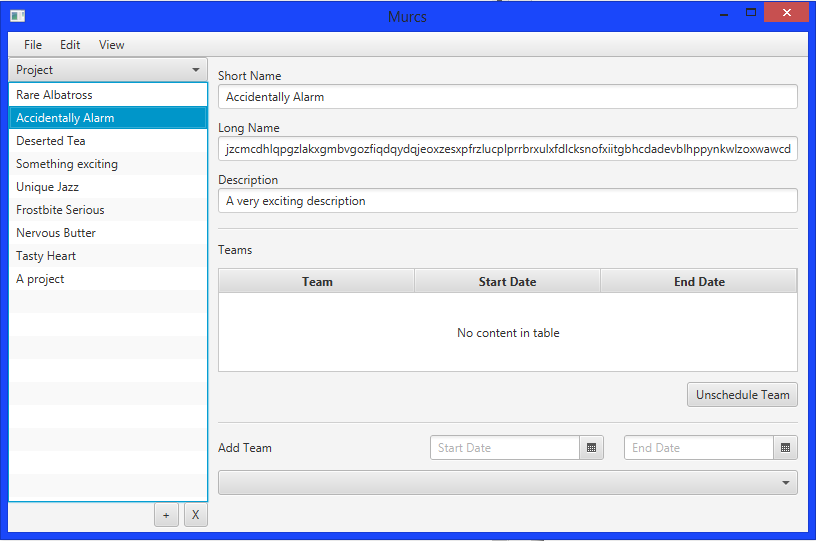
\includegraphics[width=\textwidth]{images/screenshots/teams4.PNG}
\caption{Editing a Team}
\label{fig:new_project}
\end{figure}

If at some stage you wish to delete a team then simply select it in the display list and click the X button and it will show a dialog confirming you want to delete and all the places that the team is used. If you choose to delete it then it will be deleted and removed from any of the places it is linked to other items (for instance all the people in it will become unassigned again).

\begin{figure}[H]
\centering
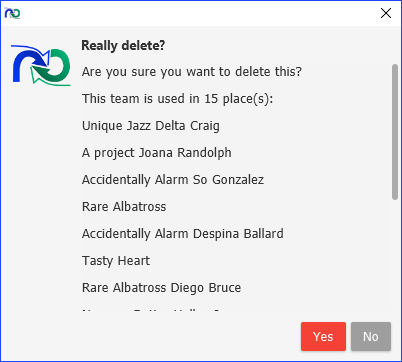
\includegraphics[width=\textwidth]{images/screenshots/teams5.PNG}
\caption{Deleting a Team}
\label{fig:new_project}
\end{figure}

For teams you can also view the number of peer programming hours and people have done within the team. If you want to see this simply go to the peer programming pane of the team editor and it will show you a list of all of the pairs of people who have worked together on every sprint the team has worked on, as shown in the figure below.

\begin{figure}[H]
\centering
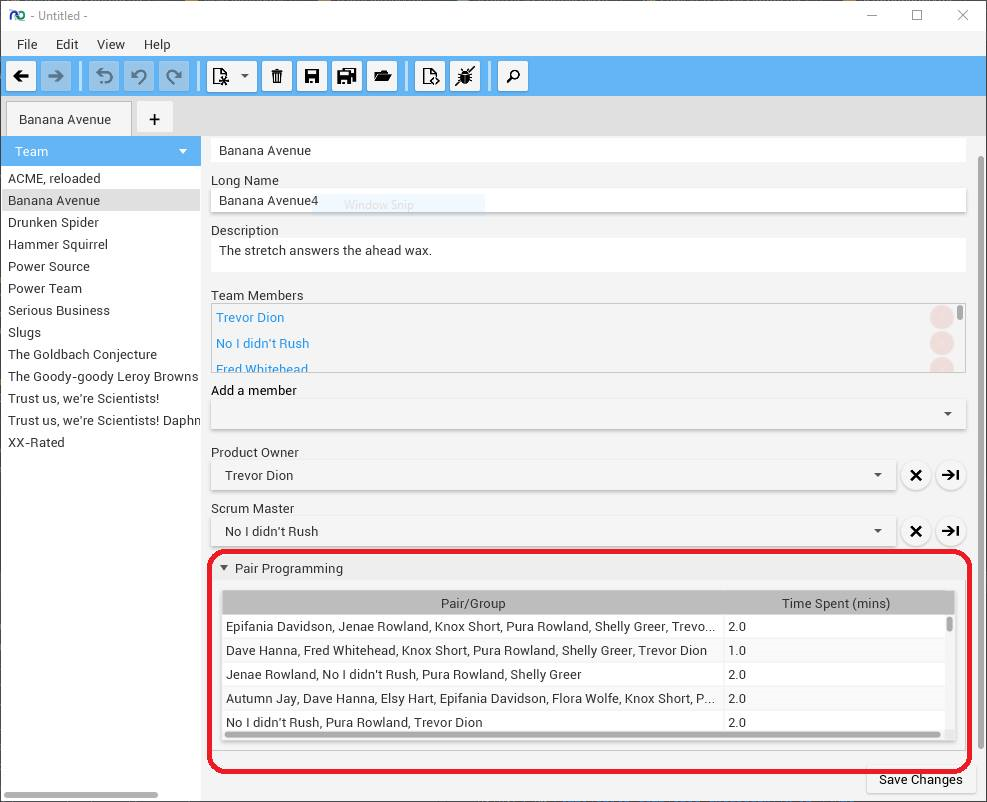
\includegraphics[width=\textwidth]{images/screenshots/teams6.PNG}
\caption{Viewing Peer Programming}
\label{fig:new_project}
\end{figure}

If you select the Velocity tab on the right, you will be presented with a chart displaying the team's velocity across all of its sprints along with their mean and median velocities. Incomplete sprints are included but are indicated as provisional.

\begin{figure}[H]
\centering
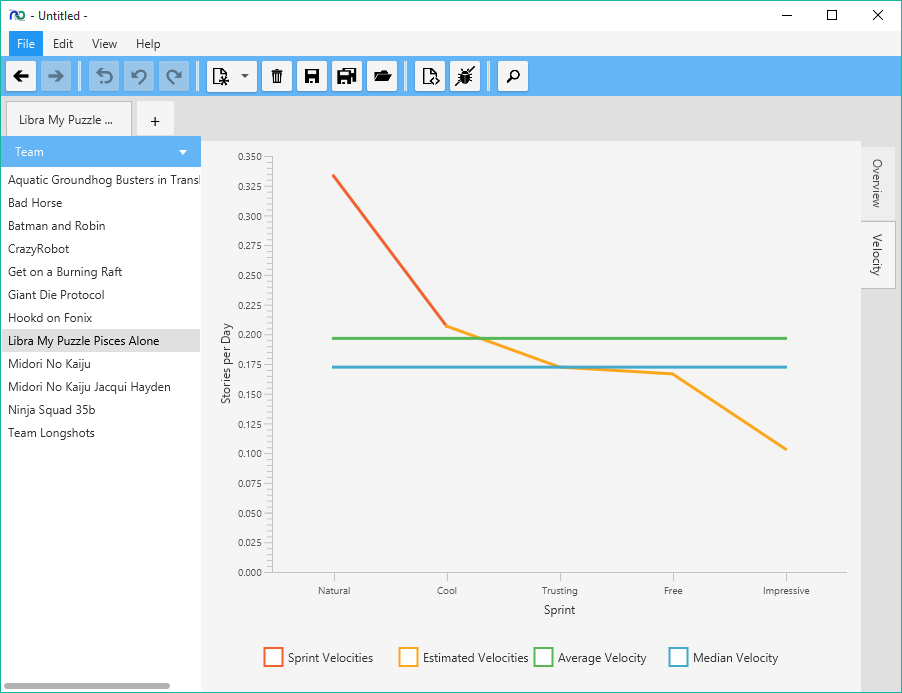
\includegraphics[width=\textwidth]{images/screenshots/velocity_board.PNG}
\caption{Velocity Board}
\label{fig:new_project}
\end{figure}